\section{Real Time 1D Computational Fluid Dynamics Simulator}
\label{sec:1dCFD}


\begin{figure}
  \vspace{-20pt}
  \begin{center}
    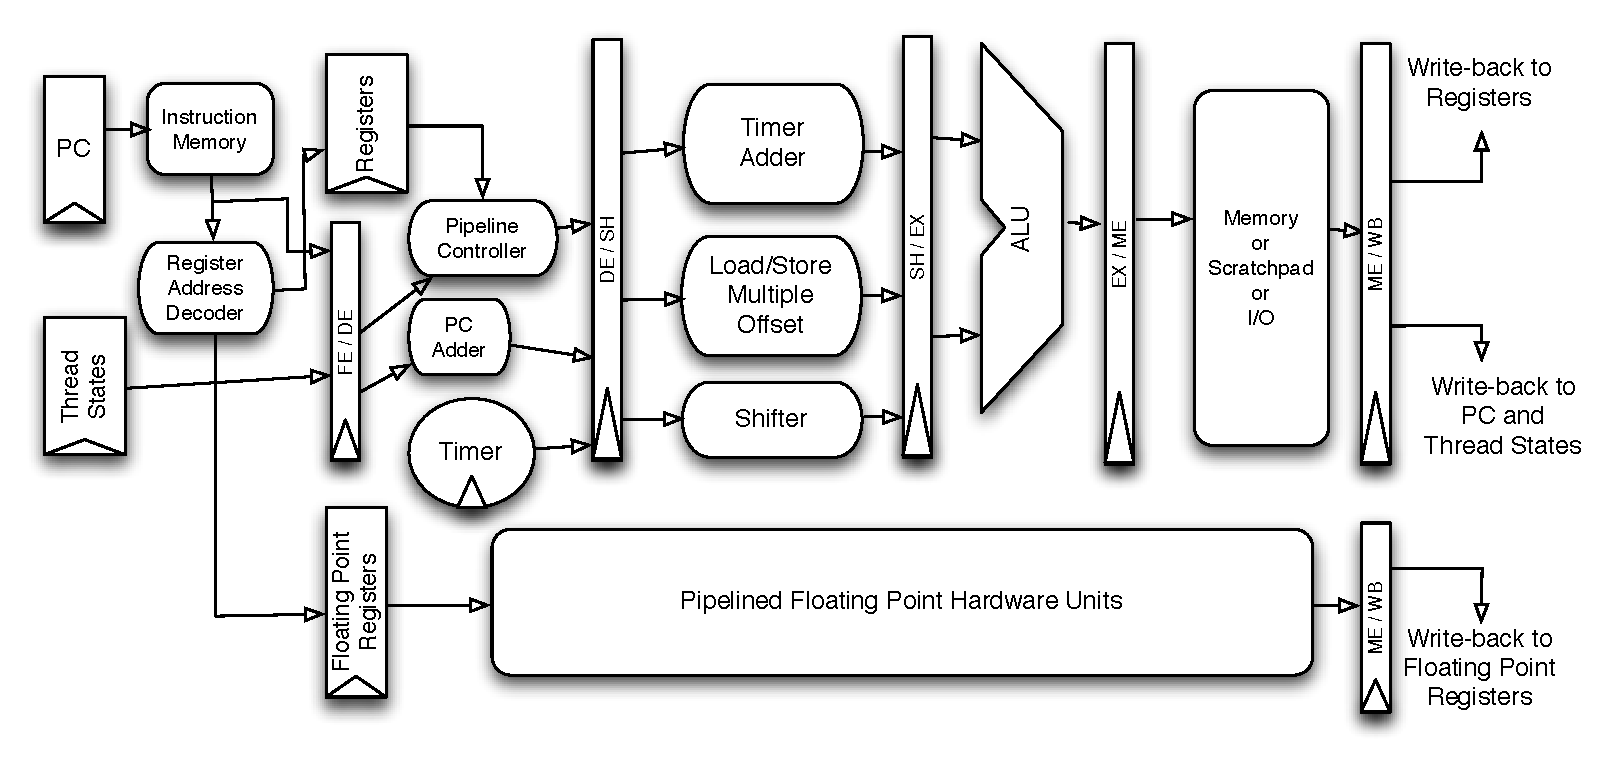
\includegraphics[scale=.6]{figs/ptarm_pipeline_six_stage}
  \end{center}
  \vspace{-20pt}
  \caption{Block Level View of the PTARM 6 stage pipeline}
  \label{fig:ptarm_pipeline_six_stage}
\end{figure}


\subsection{Introduction}
%Story - 
% 1) fuel rails are already developed and modeled using commercial 1D cfd solvers, so we can use the same technique to model in real-time, improving the efficiency of engines. 
% 2) In order to do so, we use implement 1d cfd solver by using multiple nodes to model pipe segments
% 3) For this class of problems, there is no need to optimizing performance, but instead we want to optimize on area (indirectly power)
% 4) We do so by using precision timing control hardware and software techniques, allowing us to ensure correctness and optimize on area

% \subsection{Questions}
% \begin{itemize}
% \item explain where the time step values are coming from. i.e what can be gained if we can allow faster time step?
% \item is the lock step execution part of the definition of solving the oneD cfd, or is just our way of solving it?
% \item we really don't want a related work section?
% \end{itemize}

	%\IL{Add in motivatation for the use of automation through mapping software to save on area - since we're submitting to software/hardware co-design track.}
	Diesel engines inject very high pressure diesel fuel into a combustion chamber that is full of intake air compressed to a high pressure and temperature.  
        When the diesel fuel enters the hot environment of the cylinder, it begins to combust after a short ignition delay.  Control of the valve is limited to a digital on/off command.  
        When the valve is on, fuel flows into the cylinder at a rate dominated by the pressure in the fuel rail.  
        In older style diesel engines, the ignition delay meant that all the fuel injected into the cylinder before the ignition delay would combust almost simultaneously.  
        In modern diesel engines a pilot injection is used to mitigate this.  
        The pilot injection is a small quantity of fuel that is injected ahead of the main injection.  
        The main injection is then timed to start shortly after the pilot injection has started burning, thereby eliminating the ignition delay for the main injection event and reducing audible noise.  
        In order to meet the ever tightening worldwide emissions standards, even more diesel injection pulses are commonly called for; often up to 5 pulses per cylinder event \cite{DIManual}.
	Each time the injection event happens, pulsations are sent through the fuel supply rail.  
        The high pressure, around 2000 bar, in the fuel system is often generated by a piston pump that also induces pulsations.  
        These pulses need to be damped and/or modeled before the subsequent injection event in order to ensure the correct amount of fuel is injected \cite{BoschDiesel}. 
        Currently most fuel systems use an ad-hoc model of fuel pressure for subsequent injection events \cite{Winward01082010}.
	Since many fuel rails are developed in commercial one dimensional computational fluid dynamics (1D CFD) solvers like GT-Fuel, it seems a natural approach to try use this same modeling technique to model their behavior in real-time.
        The real-time solution is necessarily rougher than the GT-Fuel calculations.
        However, if it is sufficient to allow improved fuel pressure estimation, then it can close the loop of fuel delivery, allowing for more precise air/fuel ratio control and a cleaner more efficient engine.
	This paper presents a framework for real-time execution of a 1D CFD solver on an FPGA using Precision Timed (PRET) Cores.
	  
     1D CFD is used when the system to be evaluated can be described as a network of pipes.  
     The advantage of 1D CFD over its 2D and 3D cousins is a greatly reduced number of nodes to be solved and simplified equations in each node.  
     This makes it common for use in simulating transient operation of internal combustion engines \cite{SAE2009010695}.  
     This also makes it interesting for solving these problems in real-time using a highly parallel approach.   
	We specifically examine the area of fluid flow, but heat transfer, mechanical dynamics, and electrical circuit simulation all represent similar problems.  
        In each of these problems, it may be possible to represent the set of equations to be solved as a graph where each node of the graph represents a physical quantity to be modeled, such as a sub-volume of fluid in a pipe.  
        The information path communicated by nodes is represented as the interconnect of the graph. 
%\MV{This may be covered elsewhere, move or remove}
       % If the problem can be formulated so that the number of interconnects is on the same order as the number of nodes, i.e. with N nodes the number of interconnects is much closer to N than to the triangular summation \(T_n\), then our approach is well suited.  As the number of interconnects gets large the FPGA will run out of block ram far before reaching capacity on processor cores.  
	 
	1D CFD fits into a class of problems we are calling heterogeneous micro-parallel problems. 
        The heterogeneous modifier is used to mean that there are a number of distinct node types.  Micro-parallel is used to denote small, dedicated portions of the problem being solved in each computational element. 
        This distinguishes them from homogeneous, micro-parallel problems often found in image processing, which lend themselves to GPU and SIMD solutions with large common memories \cite{10.1109/FCCM.2006.20}.
        At each time step, each node reads the neighboring data from the previous time step and computes the new data to be sent to its neighbors.
        In this periodic and parallel execution of all nodes, the performance of the system is limited by the node with the longest execution time. 
        
        It is important to understand that when modeling physical quantities, such as fluid flow, the time step is determined by the granularity of the application.  
        For an explicit solver that uses a fixed time step, it is required that the solver run faster than the speed of information flow. 
        This is expressed in equation \ref{Courant} where \(a\) is the wavespeed and \(C\) is the Courant number.  For stability the Courant number needs to be less than 1 and a number below 0.8 is recommended~\cite{GTFuel}.
\begin{equation} \label{Courant}
\frac{\Delta t}{\delta x}a = C
\end{equation}
  For instance, if a fluid has a wave speed \(a\) of 1 $cm$ per microsecond and a discretization length \(\Delta x\) of 1 $cm$, then we require a time step \(\Delta t\) of less than one microsecond.  
  This discretization length of a pipe network is dominated by its smallest sub-volume.
  For a diesel fuel system a 1 $cm$ discretization length is common.
For our purposes in this paper we treat the speed of sound (wave speed) as 1500 $m/s$~\cite{DieselSpeedOfSound}.
We require adequate performance so that the slowest node can complete in \(\Delta t\); beyond that all our optimization efforts focus exclusively on FPGA area reduction to improve scalability.
%        Improving the performance of the underlying architecture could allow us to model with finer granularity, but once the granularity is set, any attempt to improve on performance would be pointless. 
%        We simply need to ensure that the node with the longest execution time can finish its computation within the defined time step. 
%        Therefore, our optimization criteria is the hardware resources used to implement a particular graph application using our framework.
%        By optimizing hardware resources we are also indirectly optimizing the power consumption of our approach.

	The advent of caches, out-of-order executions, branch prediction, and other performance improvements in modern processors have improved their average execution speed at the cost of determinism.  
        As a result, worst-case execution time analysis often give imprecise and overestimated results. 
        For hard real-time systems this causes overprovisioning of hardware resources in order to guarantee that no timing violations occur. 
%	For hard real-time systems worst-case performance is the critical criteria. 
        The Precision Timed (PRET) Architecture~\cite{pret_cases08} is a processor architecture designed to provide timing determinism and good worst-case performance. 
        It contains multiple deterministic hardware threads, and timing instructions to gate execution time of code blocks on the hardware threads. 
        In this approach we map the heterogeneous computational nodes in the graph onto the hardware threads of multiple PRET cores. 
        The deterministic execution time ensures that each node completes within the specified time step, and the timing instructions ensure the synchronization of data communication between threads and cores.
        We show that deterministic timing allows us not only to minimize the overprovisioning of hardware, but further allows us to optimize FPGA area employed by our framework.

% 	In order to minimize the FPGA space used by this approach several optimizations were employed.  First we used multi-threaded processor cores where each processor can employ \(T\) independent hardware threads and second we optimized the layout of the graph and interconnects to minimize on processor inter-thread communication.  A further optimization we analyzed was to maximize threading on the processors\MV{We are probable not still doing this}, benchmark numbers were generated for use in later optimizations with this in place.  Lastly we employed an optimization allowing specialized hardware to be available on some processors for dedicated calculations. \MV{need to show this in the benchmarking}

% \MV{can we skip the "table of contents" below if we are out of space?}
%         In the following sections we first give some background on 1D CFD and its application to diesel engine fuel systems and the PRET architecture. 
%         Then we describe the framework used to implement the 1D CFD solver. 
%         This includes a mapping algorithm that maps distinct node types onto hardware threads to optimize for area, and the mult-core PRET architecture designed to implement the solver. 
%         We present the results of various examples that are implemented using our framework and synthesized on the Xilinx Virtex 6 FPGA. 
%         We show that by leveraging timing determinism, our framework is not only feasible but provides a scalable approach.  
%         Finally, we conclude and list some future work that is planned. 
	
%\IL{Describe PRET vs. GPU vs. Processor}
%------------------------------------------------------------------------- 

%cut out the Related Work section and place it distributed in the body

%------------------------------------------------------------------------- 
\subsection{Background}
%------------------------------------------------------------------------- 

%------------------------------------------------------------------------- 
\subsection{One-Dimensional Computational Fluid Dynamics}
\label{sec:1dcfd}
Solution of 1D CFD problems begins with the Navier Stokes equations for compressible flow.  We then build a library of solution elements for the type of pipe segments we use in the form of 1st order finite difference equations~\cite{SAE1999010915}.  
We start with momentum equation
%
\begin{equation}
\frac{P_x}{\rho}+\dot{V}+\frac{fV}{2D}|V|=0
\end{equation}
% 
and continuity equation 
%
\begin{equation}
a^2V_x+V\left(\frac{P_x}{\rho}+g\sin\alpha\right)+\frac{P_t}{\rho}=0
\end{equation} 
%
where \(P\) is pressure, \(\rho\) is fluid density, \(V\) fluid velosity, \(f\) is the Darcy-Weisbach friction factor, \(D\) is pipe diameter, \(a\) is the wavespeed, and \(g\sin\alpha\) is the directional force of gravity.  A dot ( \(\dot{ }\) ) over a variable indicates the total derivative with respect to time and the "\(_x\)" and "\(_t\)" subscripts indicate partial differentiation along the pipe length and with respect to time. 

These equations can be expanded and simplified by leaving out the body force and convective terms because these are negligible given the pressure and flow regime.  This leads us to the following equations in the form \(L=L_1+\lambda L_2\):  
%
\begin{equation}
L_1=\frac{P_x}{\rho}+V_t+\frac{f}{2D}V|V|=0
\end{equation} 
%
and 
%
\begin{equation}
L_2=\frac{P_t}{\rho}+a^2V_x=0.
\end{equation}

A method of characteristic solution is used to explicitly evaluate the pressure and flow at the next step through a first order finite difference method.  Figure \ref{Interp} 
shows the evaluation of pressure and flow at point \(I, t_0+\Delta t\) based on the pressure and flow of the adjacent points at time \(t_0\).  The equations to be evaluated at each point are
%
\begin{align}
V_{I}= & 0.5\left[V_{i-1}+V_{i+1}+\frac{1}{a\rho}\left(P_{i-1}-P_{i+1}\right) \right. \nonumber \\
	& \left. -\frac{f\Delta t}{2D}\left(V_{i-1}|V_{i-1}|+V_{i+1}|V_{i+1}\right)\right]
\end{align}
%
and
%
\begin{align}
P_{I}= & 0.5\rho \left[\frac{1}{\rho}P_{i-1}+P_{i+1}+a\left(V_{i-1}-V_{i+1}\right) \right. \nonumber \\
	& \left. -\frac{af\Delta t}{2D}\left(V_{i-1}|V_{i-1}|+V_{i+1}|V_{i+1}\right)\right].
\end{align}

One critical part in evaluating the value at point \(I\) is that there is a fixed relationship between \(\Delta x\), \(\Delta t\), and the wave speed \(a\) such that \(a=\Delta x/\Delta t\).  \(\Delta x\) is fixed by the geometry of the problem and \(a\) is fixed by the properties of the working fluid such as \(a=\sqrt{K/\rho}\), where \(K\) is the bulk modulus. 
Therefore, our \(\Delta t\) is defined for us.  
All of our computations must be complete within \(\Delta t\) and the results must be posted at exactly \(\Delta t\).  Because the wave speed varies and the geometry of the problem may not work out evenly for all pipe segments a modified method is implemented with an interpolation step.  This is shown in Figure~\ref{Interp} and described by equations
%
\begin{equation}
\zeta_R=\zeta_C-\theta a(\zeta_C-\zeta_A) \text{ and}
\end{equation}
%
\begin{equation}
\zeta_S=\zeta_C-\theta a(\zeta_C-\zeta_S).
\end{equation}
%
where \(\theta\) represents the amount of interpolation desired.
These equations are evaluated for both pressure \(\zeta = P\) and velocity \(\zeta = V\).
While we use this method to give our calculations leeway it is important to realize that this adds complexity to every block in the system as well as decreasing the \(\Delta t\) we have to work with.  
%Using this method does not reduce the precision required in posting the results every time step.
%
\begin{figure}  
\centering 
\includegraphics[width=0.4\textwidth,page=10]{./figs/1dcfd/ElementalProcessors.pdf}
\caption{First Order Difference} 
\label{Interp}
\end{figure}

In order to evaluate our system of pipes we define a few types of computing nodes that corresponding to different pipe elements.  Specifically, the types are:
%\begin{enumerate}
%\item
1)~Pipe Segment;
%\item 
2)~Imposed pressure upstream, representing the pressure sensor on the fuel system;
%\item
3)~Imposed mass flow into the pipe, representing a pump;
%\item
4)~Valve at downstream end of pipe, representing an injector;
%\item
5)~Cap at downstream end of pipe;
%\item 
and 6)~``T" intersection.
%\end{enumerate}
%
Different types of computing nodes execute different algorithms on the same hardware.  

Rearranging the equations again and making the substitutions \(B = a\rho / A\) and \( R=\rho f \Delta x/2DA^2\), where \(A\) is the cross sectional area of the pipe, and \(Q\) is the flow rate along the pipe, we get the simplified characteristic equations
%
\begin{equation}
C_P=P_{i-1}+Q_{i-1}\left(B-R|Q_{i-1}|\right) \text{ and}
\end{equation}
%
\begin{equation}
C_M=P_{i+1}-Q_{i+1}\left(B-R|Q_{i+1}|\right).
\end{equation}
%
%With this notation the solution for a generic pipe section is
%
%\begin{equation}
%P_{I_n}=\frac{\left(C_P+C_M\right)}{2} \text{ and}
%\end{equation}
%
%\begin{equation}
%Q_{I_n}=\frac{\left(P_{I_n}+C_m\right)}{B}.
%\end{equation}

Table \ref{types} shows the equations for each of the supported pipe elements.  From these pipe elements we can generate a network of pipes that represent our fuel system.  
%
\begin{center}
\begin{table}
\caption{Equations for Supported Types} 
\begin{tabular}{|c|c|c|}
\hline
Type 							&$P_{I_n}=$ 										&$Q_{I_n}=$ \\ 
\hline
Pipe Seg. 						&$\frac{\left(C_P+C_M\right)}{2}$ 				&$ \frac{\left(P_{I_n}+C_m\right)}{B}$ \\ 
\hline
Imp. P 							&$\scriptstyle P_{Bnd}$ 							&$\frac{(P_{Bnd}-C_M)}{B}$ \\
\hline
Imp. Q 							&$\scriptstyle C_M+BQ_{Bnd}$ 					&$ \scriptstyle Q_{Bnd}$ \\
\hline
\multirow{3}{*}{Valve} 		&\multirow{3}{*}{$\scriptstyle C_P-BQ_{I_n}$}	&$\scriptstyle -BC_V+\sqrt{(BC_V)^2+2C_VC_P}$ \\ 
 								&													&$\scriptstyle C_V=\frac{(Q_0 \tau)^2}{2P_0}$\\ 
\hline
Cap 							&$\scriptstyle C_P-BQ_{I_n}$ 					&$\scriptstyle 0$ \\ 
\hline
\multirow{3}{*}{Pipe ``T"} 	&\multirow{3}{*}{$\frac{\frac{C_{P_1}}{B_1}+\frac{C_{M_2}}{B_2}+\frac{C_{M_3}}{B_3}}{\sum \frac{1}{B}}$} &$-\frac{P_I}{B_1}+\frac{C_{P_1}}{B_1}$ \\ 
 								&  													&$-\frac{P_I}{B_2}+\frac{C_{M_2}}{B_2}$\\ 
 								& 													&$-\frac{P_I}{B_3}+\frac{C_{M_3}}{B_3}$\\ 
\hline
\end{tabular}
\label{types}
\end{table}
\end{center}

%------------------------------------------------------------------------- 
\subsection{Precision Timed Architecture}
\label{sec:PRET}
% Most modern computer architectures are designed to improve average case performance by trading off worst-case performance. 
% For example, caches improve memory access latencies by pre-fetching memory contents into a local faster memory. 
% But a wrong prediction of what memory contents the processor needs (cache miss) results in a longer memory latency due to the miss penalty.      
% \MV{This is repeated almost exactly from the intro, consider cutting one if we are short on space}
For real-time applications that need timing determinism, Edwards and Lee~\cite{Edwards:2007} propose Precision Timed (PRET) Architectures. 
These are architectures design for timing predictability and determinism, rather than average case performance. 
Lickly et al.~\cite{pret_cases08} present a multi-threaded implementation of the PRET architecture using a thread-interleaved pipeline and scratchpads.  
The thread-interleaved pipeline removes data and control hazards within the pipeline by interleaving multiple hardware threads in a predictable round robin fashion.
%\MV{Mention that these are ARM cores, specifically which version of ARM or what makes it different from say a generic ARM9.  Mention that code was complied with GCC with what optomiztion settings}
Scratchpad memories are single-cycle access on-chip memories which are managed in software. 
It is typically used in place of a cache to improve on predictability because the contents on the scratchpad is transparent in software. 

Along with the predictable architecture, Lickly et al.~\cite{pret_cases08} also introduce an instruction to control the temporal behavior of programs.
The deadline instruction, as named in the paper, gives programmers a way to specify a lower bound on execution time for a specific code block, guaranteeing that a code block will not finish early.
%, thus ensuring determinism.
%Although it may seem counter intuitive to specify a lower bound on execution time, it is quite useful in reality. 
%One example is of how this instruction could be used is to achieve mutual exclusion for shared data amongst multiple threads. 
%Mutual exclusion typically requires mutexes or locks to ensure only one thread accesses the shared data at a time. 
%But locks and mutexes make no guarantee on the time it takes to acquire the lock, or which thread currently has the lock. 
%This makes execution time extremely unpredictable, and possibly dependent on the execution state of other threads.   
Lickly et al.~\cite{pret_cases08} outlined a producer consumer example that synchronizes communication through the use of deadline instructions to ensure an ordering between shared data access. 
Our implementation of the 1D CFD solver leverages this instruction to synchronize communication across computational nodes and align the computation with real-world events. 

%------------------------------------------------------------------------- 
\subsection{Framework}
\subsection{System Description and Design Flow}

In order to design and implement our system we must go through the following steps:
\begin{enumerate}
	\item Define the problem class as a library of computational elements.
	\item Develop the thread code for each element.
	\begin{enumerate}
		\item Determine worst-case timing.
		\item Add or remove processor hardware to optimize elements for speed and area.
	\end{enumerate}
	\item Map the specific problem in to a graph of where each node of the graph is represented by an element of the library.
	\item Determine the time available for each time step to determine the number of threads per core.
	\item Optimize core grouping and interconnect.
	\item Compile for the target FPGA.
\end{enumerate}

%To make practical use of our system we need to connect it to a real-world application.  
Figure \ref{HighLevelDiagram} shows an overview of a representative system for modeling fuel rails.  
%
\begin{figure}
\centering
\includegraphics[page=7, width=0.4\textwidth]{./figs/1dcfd/ElementalProcessors.pdf}
\caption{High Level System Diagram}
\label{HighLevelDiagram}
\end{figure}
%
The 1D CFD model is bounded inside the dashed rectangle.  
External to that is the real-word sensor and actuator interfaces that provide boundary conditions or consume model output variables.  
The small blue squares inside the dashed rectangle represent the network of pipes.  
In a practical simulation of a diesel fuel system the total number of pipe elements can range from around 50 to a few hundred.  

Each pipe element is a computational node, and their graphical representation is shown in Table~\ref{CELibrary}. 
The top 3 rows of the table represent the pipe elements described in Table~\ref{types}.  
%The 4th row contains two helper functions that also run on threads of processors.  
Mechanical calculation elements compute the inputs to valve, defined flow and defined pressure blocks.
They serve as an interface between the flow model and the real world.
Global calculation elements are used to compute the temperature dependent variables of density and wave speed. 
They post their data to a global distribution block, broadcasting it to all nodes.
Blocks with white backgrounds denote that they are implemented directly in FPGA fabric, not mapped to a processor thread.  
The Global Distribution node is purely used to indicate a distribution of input value to each of the computational elements in our model. 
The Display node is used when data needs to be communicated out of the model through a register or FIFO to other parts of the FPGA. 

For illustrative purposes, we show a simplified sample pipe network with a imposed flow input in figure \ref{DetailedDiagram}. 
Fluid travels through a few pipe segment nodes to a ``T" intersection, where it splits off to a second branch of the network.
The ``T" node is also measured by the outside world through a display port.  
Flow going up the new leg ends in a cap, while flow continuing down the original path exits the system through a valve.  
The system is assumed to be at uniform temperature and values based on the temperature dependent variables of density and wave speed are delivered to each of the computational elements every time step for use in the subsequent time step.
For the purposes of system analysis we assume that flow always enters through the left and exist to the right and possibly top of the network element.  This lets us describe the system as a directed graph of the form in Section \ref{sec:mapping}. 
%Since global values are delivered to every node they may be omitted from our graph representation.
%

%
\begin{table}
\begin{center}
\caption{Library of Computational Node Elements}
\begin{tabular}{|p{2cm}|c|p{2cm}|c|}
\hline
Pipe 			&\includegraphics[page=11, scale=0.25]{./figs/1dcfd/ElementalProcessors.pdf} &
Cap 			&\includegraphics[page=12, scale=0.25]{./figs/1dcfd/ElementalProcessors.pdf} \\ \hline
Imposed Pressure 			&\includegraphics[page=13, scale=0.25]{./figs/1dcfd/ElementalProcessors.pdf} &
Imposed Flow 			&\includegraphics[page=14, scale=0.25]{./figs/1dcfd/ElementalProcessors.pdf} \\ \hline
Pipe ``T" 		&\includegraphics[page=15, scale=0.25]{./figs/1dcfd/ElementalProcessors.pdf} &
Valve 			&\includegraphics[page=16, scale=0.25]{./figs/1dcfd/ElementalProcessors.pdf} \\ \hline
Mechanical Calc.	    &\includegraphics[page=17, scale=0.25]{./figs/1dcfd/ElementalProcessors.pdf} &
Global Calc. 	&\includegraphics[page=18, scale=0.25]{./figs/1dcfd/ElementalProcessors.pdf} \\ \hline
Global Dist. 	&\includegraphics[page=19, scale=0.25]{./figs/1dcfd/ElementalProcessors.pdf} &
Display 		&\includegraphics[page=20, scale=0.25]{./figs/1dcfd/ElementalProcessors.pdf} \\ \hline
\end{tabular}
\label{CELibrary}
\end{center}
\end{table}


%
\begin{figure}
\centering
\includegraphics[page=3, width=0.4\textwidth]{./figs/1dcfd/ElementalProcessors.pdf}
\caption{Detailed System Diagram}
\label{DetailedDiagram}
\end{figure}
%

\subsection{Hardware Architecture} 
\label{sec:hardware_architecture}
The hardware architecture consists of multiple PRET cores connected through point-to-point connections and a global distribution circuit.
Figure~\ref{ARM_Cores} shows a block-level view of the hardware architecture.   
As mentioned in Section \ref{sec:PRET}, each core consists of hardware threads interleaved through the pipeline in a predictable round robin fashion.
Thus, computational nodes are mapped onto hardware threads, instead of implemented as its own core.
%This saves on the resources required for each node to implement its own dedicated datapath.  
This provides two major advantages.  
First, multi-threaded architectures maximize the throughput over latency.  
The thread-interleaving can utilize pipelined ALUs and floating point units to make normally multi-cycle instructions appear as single-cycle instructions when timing analysis is done on individual threads. 
%Normally multi cycle instructions could now appear to be single-cycle when doing timing analysis on individual threads. 
In our implementation, all floating point operations except square root and divide appear as single-cycle instructions during timing analysis.      
%pipelined instructions like divide can appear as single step instructions to their respective thread.  
%Further space savings can be achieved by pipelining instructions, like add, that would not normally be pipelined, though we do not examine this in our benchmarks.\MV{Isaac, is what I said here true?}
Second, the thread interleaved pipeline design allows for a simpler pipeline design.
Since data and control hazards are no longer present in the pipeline, the logic used for handling them can be stripped out, greatly reducing the cost of the core.
Furthermore, multiple threads share the same datapath, so the cost of adding threads is far less than adding a core, further reducing the cost of the system.
We discuss in more detail the trade-offs involving adding threads in Section~\ref{sec:results}.
%IL{Talk about how different hardware resources can be synthesized}
The memory footprint required for each node is small enough (roughly a hundred instructions) that the scratchpad is sufficient for memory use, no main memory is needed.

Only basic single-precision floating point operations (add/sub/multiply) are needed for most nodes, but some require more complicated operations;  
the valve element uses floating point square root and the ``T" element uses floating point divide.
However, these elements typically represent only a few percent of the overall system.  
In our complex example, the common rail fuel system, there are 234 nodes; only 5 nodes are ``T"s requiring division and 4 node are valves requiring square root.
To save on hardware resources, we could use software emulation for the complex operations. 
%This way we don't need to synthesize extra hardware for each core, which would only be used by the small percent of nodes that need it.  
However, our system is bounded by the slowest computational element, so the performance hit from using software emulation for these small percent of nodes would limit the overall performance of our system. 
But if we decide to add hardware units on the core, it would go wasted on most cores with a homogeneous multicore approach.
%In a homogeneous core approach, we would need to add hardware units to all cores if we required the performance for the few nodes. 
Instead, we adopt a heterogeneous multicore approach and provide several configurations of our core that includes different floating point hardware units.
The mapping algorithm described in Section~\ref{sec:mapping} uses this to optimize the resources used in the system by grouping nodes with similar functionalities onto the same core. 
We only synthesize hardware accelerators to the cores that need them. 
Since this number is small, we still get the throughput improvement from adding hardware support without the huge resource overhead. 
This proves to provide substantial resource savings, which we show in Section~\ref{sec:results}.  

%our approach adds hardware support for square root and divide only to the cores that contain a valve or ``T'' element.
%We describe in more detail the optimization and mapping algorithm in section~\ref{sec:mapping}. 
\begin{figure}
\centering
\includegraphics[page=8, width=0.4\textwidth]{./figs/1dcfd/ElementalProcessors.pdf}
\caption{System of Multithreaded PRET Cores and interconnects}
\label{ARM_Cores}
\end{figure}

%The heterogeneity of the nodes allows us to configure the cores according which nodes are mapped onto the cores. 
%\IL{Talk about different features for the core - floating point, fixed point, square root, divide} 
%We show in section~\ref{sec:results} the resources used for the different configurations of our core.
 
Each node in our system requires four input ports along with output ports connected to its neighboring nodes.  
%The input ports are labeled "Left", "Right", "Top", and "Global" by default though they are overloaded as necessary for specific functions, for instance the valve node uses the top port to input valve position.
One input port is dedicated as the global port, which always receives broadcasts from the global distribution circuits.
Since only local communications occur across nodes, only point-to-point communication channels need to be established. 
A complicated interconnect between all cores is not needed. 
%We only need to establish point-to-point communication channels between a core and its neighbors to ensure communication for the nodes mapped on the threads.
Nodes mapped to the same core (intra-core communication) can communicate through the shared local memory within the core.
Nodes mapped to different cores (inter-core communication) communicate through the point-to-point interconnect.  
We use shared dual-ported Block RAMs (BRAM) for our inter-core communication.
This serves two purposes. 
First, it provides single-cycle deterministic communication.
This allows the timing analysis to be simplified, as there is no hardware protocol that needs to be accounted for when accessing data through the inter-core communication channels. 
More importantly, the timing analysis for each node is now independent of the node mapping; both intra and inter core communication mechanisms are single-cycle. 
If this were not the case, then the timing analysis needs to assume all communications are inter-core communications, the longer of the two. 
Second, by using the dedicated BRAM blocks on the FPGA for interconnects, we save the logic slices to be used for computation nodes.
This is useful because the limiting resource in our implementation is logic slices, not BRAMs. 
%BRAM blocks are specialized resource blocks on the FPGA that are used to synthesize fast memory.
Each core only requires a small number of BRAMs to be used for registers and scratchpads, so the BRAM utilization ratio is far less than the logic slice utilization ratio.
At each time step only two words, pressure and flow rate values, are being transferred from a node to each of its neighbors. 
Our periodic software model (described in Section~\ref{sec:software_architecture}) ensures that we only need a buffer size of one for each of the words. 
Because the communication bandwidth is small, we only need one BRAM block to establish an interconnect that allows all threads from one core to communicate with all threads on the other.

%By using precision timing to achieve data synchronization, this allows us to use simple hardware mechanisms such as a single BRAM to establish a single buffer for communication while ensuring no data races between nodes.   
%\IL{Make sure to explain why you don't need handshaking protocols in hardware, because we're doing it in software}  

%In our diesel fuel system implementation we assume all nodes are at the same temperature and compute the temperature dependent parameters wave speed and density globally.  
%Our system derives 3 temperature dependent parameters in an optimized form, and broadcasts them to every pipe element.   
All of our pipe elements have a dependency on density and wave speed that are functions of temperature.  
Temperature is assumed to be the same throughout the system, so these parameters are computed in a single computational element and broadcast to all pipe elements through the global distribution circuit.
%For the global distribution circuit, we observe that most nodes only need to receive the broadcast; only a few nodes are sending the broadcast.  
%In fact, in diesel fuel systems, the number of parameters that need to be broadcast can always be fitted into a single core \IL{Matt, is this valid assumption? Is there a better way to state this?}.
%These 3 parameters are delivered to every pipe element.
Leveraging this, the global distribution circuit is implemented by a single broadcast bus with one master that writes to dedicated memories local to each core.
This broadcast receiving memory is synthesized to a small dual ported BRAM, with a read-only side connected to the core, and a write-only side connected to the bus.
This memory is shared amongst all threads in a core so all threads can access the global values.
% of an extra dual ported BRAM at each core.
%All  and a single broadcast bus with that allows a dedicated core to write to the small local buffers.
The bus master is a also dedicated PRET core that global calculation nodes map to. 
Since the broadcast mechanism involves only sending a BRAM write command through the broadcast bus, it is only a single-cycle operation, as the broadcast receiving memories can all receive the broadcast and write in the broadcast values within a single cycle.
%The buffer can only be written from the broadcast bus and is read-only from the cores.
%The small local buffers are memory mapped on each core and can be accessed by all threads on the core.
%The mapping algorithm described in section \ref{sec:mapping} ensures that nodes which require global broadcasting of data will be mapped to a thread on the dedicated broadcast core.
This implementation allows us to save on the resources needed to implement a full fledged interconnect routing system or any network protocol to be used for broadcasting. 

%On the left you can see a six-thread implementation of the basic PRET architecture where each thread has its own register set and shares the pipelined ALU and more memory in a time-sliced fashion.  
%Additional cores are shown in smaller scale on the right.  
%Data connections between cores are shown with solid arrows.
  
%In this simple diagram data connection is shown only from one core to the next in a clockwise fashion around the diagram.  
%In more complex situations each core can be connected to between one and all other cores in the system, but as the amount of interconnection increases the advantages of this model over a global memory model decrease. \IL{This is not true actually, managing a global memory when core numbers go up is very costly.}

%In order to optimize FPGA resources we look at the relative costs in FPGA gates of various components in the system.  
%First is the cost of additional threads per processor core. 
%In our implementation we used a 150MHz system clock speed with 6 threads, so this is our baseline for area in Table \ref{Cores_vs_features}.  
%This is then divided by the number of threads to get the virtual execution rate of the cores.  

%\GW{are these number with div or not???}

%The additional cost of the global interconnect was neglected because the majority is built into the estimated cost of the cores. 
%The costs of the interconnects themselves are \MV{insert num} based on the weighting in Table \ref{Cores_vs_features} but significant because the number of interconnects can far exceed the number of cores.  
%It is important to note that due to the structure of block RAM in the Xilinx FPGAs examined there is a minimum size that is adequate to transport all parameters from a given core.  
%This means that once a core to core interconnect is established (and edge on the graph) all additional interconnect between various threads on those cores comes for free.


% %
% Each of these computational elements represented in the library is instantiated on one thread of one of the processor nodes.  
%------------------------------------------------------------------------ 
\subsection{Software Architecture}
\label{sec:software_architecture}
We implement the equations from Table~\ref{types} in C and compile it with the GNU ARM cross compiler~\cite{gnu-arm} to run on our cores. 
% In order to minimize the computation required, the equations are statically optimized.  
% The system is also assumed to be at a constant temperature measured by an external sensor.  
% The temperature dependent terms of wave speed and density are computed globally and passed to each of the nodes each time step. 
Columns 2-6 in Table \ref{InstructionCount} show the number of Add/Subtract, Multiply, Absolute Value, and Square Root operations required by each computational element after optimization, neglecting the interpolations operations.
The computation for each node is executed in parallel on multiple threads and synchronized each time step.
Data is exchanged only at the boundaries of the time steps to avoid data races. 
Each time step consists of three phases for the computational pipe elements:
\begin{enumerate}
  \item Reading in the pressure and flow rate values from neighbors, and read in global values.
  \item Compute the output value.
  \item Send output values to neighbors to be used for next time step.
\end{enumerate}
The global and mechanical nodes do not need to read data from other nodes, but might gather data from physical sensors and broadcast or send data to other nodes.  
Figure~\ref{fig:software_model} shows a rough timeline view of the operations for each node.    

\begin{figure}
\centering
\includegraphics[width=0.45\textwidth,page=5]{./figs/1dcfd/ElementalProcessors.pdf}
\caption{Execution of nodes each time step}
\label{fig:software_model}
\end{figure}
There are several software implementations for a periodic execution model, but the execution time analysis of each node is crucial to ensure that we can meet the timing constraints imposed. 
%Our implementation leverages the PRET architecture to ensure periodic execution with low overhead.
%Although , any complex software control structure would still require path exploration or loop bound analysis for accurate time analysis.
The computation done by each node consists only a single path of execution, voiding the need for complex software analysis.
The PRET architecture provides a precise architectural timing analysis, which can provide exact execution time for single path executions.     
%If mutex or locks were used to synchronize communication, the complexity of timing analysis would greatly increase because the execution time would be heavily influenced by the actions of other threads. 
Data synchronization is handled by the synchronized periodic execution of nodes, which enforces an ordering between the writing and reading of shared data.
This voids the need of any explicit synchronization methods, and allows all inter and intra core read, write, and broadcast operations to be single-cycle operations as described in the previous section. 
%So reading and writing across nodes in our implementation are simply reads and writes to memory mapped locations. 
%Broadcasting data to all nodes is also implemented by writing to a specific memory address region. 
%As described in the previous section,   
These properties allows us to statically obtain an exact execution time for each computation node, which we show in the last two columns of Table~\ref{InstructionCount}. 
The execution time is measured in thread cycles, defined by the number of times the thread is fetched into the pipeline. 
To convert the thread cycles to physical time, multiply the thread cycles by the number of threads to get clock cycles, then convert the clock cycles to physical time according to the processor clock speed.  

In addition to statically assuring that the worst-case execution time meets the timing constraints specified, we also need to enforce that node executions remain synchronized.
Our approach uses specialized timing instructions provided by the PRET architecture to enforce a lower bound execution time of code segments.
By enforcing a lower bound execution time that is greater than the worst case, we enforce all nodes to take exactly the same amount of time to execute, thus keeping them synchronized.
%The overhead of these instructions is very low, as they are designed directly into the core~\cite{pret_cases08}.
Figure \ref{fig:software_model} shows the program synchronization points which our timing instruction enforces.
The grayed area in the figure denotes slack time that is generated by the timing instructions.
We insert one instruction at the beginning of each block to specify the minimum execution time, and one instruction at the end to enforce it.
When the latter instruction is decoded, the program will wait until the minimum time is exceeded, then continue execution.
Each timing instruction takes 2 cycles because it is manipulating 64 bit values representing time. 
For our computational elements, 6 instructions are used in the main loop, thus 12 cycles of overhead is introduced per time step.
These are already included in our execution time analysis presented in Table~\ref{InstructionCount}. 
The same effect can possibly be achieved with no overhead using instruction counting and NOP insertions.
This can certainly be done on any deterministic architecture such as PRET. 
However, NOP insertion is both brittle and tedious. 
Any change in the code and insertions needs to be redone to ensure the correct number of NOPs are added.
Designs now are mostly written in programming languages like C and compiled into assembly, making it extremely difficult to gauge the number of NOPs needed at design time.
The timing instructions allow for a much more scalable and flexible approach. 
In a system with heterogeneous nodes and different execution times, the timing instructions allow us to set the same deadlines in all nodes regardless of its execution time.   

%Each timing instruction takes 2 thread cycles, and allows timing control at granularity of thread cycles.     
%Its precision however is at the order of tens of nanoseconds, providing a high precision at extremely low cost. 
%\IL{Rework a little the part on timing instructions}

\begin{center}
\begin{table}
\caption{Computational Intensity of Supported Types}
\begin{tabular}{|c|c|c|c|c|c|c|c|}
\hline
\multirow{2}{*}{Type}	&\multirow{2}{*}{Mul}	&Add/	&\multirow{2}{*}{Abs}	&\multirow{2}{*}{Sqrt}	&\multirow{2}{*}{Div}	&\multicolumn{2}{c|}{Thread cycles} \\ \cline{7-8}
 			& 		&Sub 	& 		&		&		&w/interp	&w/o \\ 
\hline \hline
Pipe Seg.	&10 	&5 		&2		&0 		&0		&  91		& 74 \\ 
\hline
Imp. P 		&6 		&3 		&1		&0 		&0		&  76		& 61 \\ 
\hline
Imp. Q 		&5 		&3 		&1		&0 		&0		&	77		& 63 \\ 
\hline
Valve 		&13 	&5 		&1		&1 		&0		&	97		& 79 \\ 
\hline
Cap 		&4 		&2 		&1		&0 		&0		&	71		& 60 \\ 
\hline
Pipe ``T" 	&16 	&13 		&3		&0 		&4		&	114		& 98 \\ 
\hline  
\end{tabular}
\label{InstructionCount}
\end{table}
\end{center}

%------------------------------------------------------------------------ 
\subsection{Mapping Optimization}
\label{sec:mapping}

	Appropriately mapping a given problem to hardware resources is an important step ensuring that the FPGA device will be used efficiently. Here we present a preliminary mapping algorithm that optimizes resource usage.
	  
%------------------------------------------------------------------------
%\subsubsection{Mapping Computational Graph to Processing Elements}
The 1D CFD real-time simulation can be described as a directed graph $G=(N,E)$, where $N$ is the set of computational nodes and $E$ is the communication among them. E.g., $e = (n_1, n_2) \in E$ means node $n_1$ sends data to node $n_2$. 
%
%Notice that at this level communication is always described between computational nodes . 
At the implementation level, computational nodes are mapped to cores that execute the real-time 1D CFD. 
%At this level, communication is further categorized as intra-core communication and inter-core communication. The former captures the communication among the threads mapped to a single core while the latter serves communicating threads that are mapped to different cores.
Each core consists of a fixed number of threads that are simultaneously running on it. 
The cost of a core is fixed and includes both resources for performing computation and intra-core communication among the set of threads mapped to this core. 
%Since there usually exists more computational nodes than the number of threads that a core can handle, some communicating thread pairs will have to be mapped onto different cores and their communication needs to be served through inter-core communication channels. 
Inter-core communication also introduces an fixed cost. However, once communication is established between two cores, any thread mapped onto one of them can freely talk to its communicating thread that is mapped onto the other. 
All the computational nodes need to be mapped onto PRET processor cores on the FPGA. 

This mapping problem is defined as follows:
%
\begin{equation*} \label{eq:DG}
\mathcal{M}: N \rightarrow C,
\end{equation*}
%
where $N$ is the set of computational nodes and $C$ is the set of cores that needs to be synthesized to perform the 1D CFD simulation. 

There exist many different optimization techniques to map a real-time graph evaluation to physical computational resources, but their resource usage may be different. 
For example, fully taking advantage of the thread capacity on a core can reduce the number of cores needed to fulfill the simulation task.
 %by cores since this will use as few cores as possible to fulfill the simulation task. 
Conversely, abusing inter-core communication because of a poor mapping which introduces immense communication between cores may increase cost tremendously. 
Instead, we want to leverage the fact that once an interconnect is established for a fixed cost, it is established for all threads from one core to the other.
Thus, if mapping a computational node requires inter-communication to its neighbor, then we want to map other nodes that can use the same inter-communication channel onto the same two cores respectively.  
%When communication between two cores is needed and established via computational nodes previously mapped onto them, 
%we want to take full advantage of this inter-core communication channel by mapping other communicating nodes onto these two cores respectively.
 
%We formulate the mapping problem as an optimization problem based on integer linear programming.
%------------------------------------------------------------------------
\subsubsection{Optimization Algorithm}
\label{sec:opt_alg}

The above mapping problem can be formulated as an optimization problem as follows. 
%Given a computational graph $G=(N,E)$ (the real-time constraints have already been respected when generating $G$, in other words, the number of computational nodes and the connectivity among them are determined by the real-time constraints), our optimization problem is to synthesize a set of cores $C$ to perform the real-time simulation and to find the optimal mapping, that is a mapping from computational nodes to the set of synthesized cores with the minimum implementation cost.
Given a computational graph $G=(N,E)$, the number of computational nodes and the connectivity is determined by the real-time constraints.
Our optimization problem is to synthesize a set of cores $C$ to perform the 1D CFD simulation in real time and to find the optimal mapping, that is a mapping from computational nodes to the set of synthesized cores with the minimum implementation cost.

In this formulation, we assume that cores are functionally heterogeneous. 
Specifically for the application we are targeting as shown in Table~\ref{InstructionCount}, square root and division computation are needed only by a few computational nodes. 
To save resources, cores with the operation of square root or division are instantiated only when this operation is needed. 
In our application, there exist four types of cores: a basic core, and three special cores: a square root core, a division core, and a core that contains both. 
Let the cost of a base core be $U$, the extra cost due to square root, division, and square root plus division be $\Delta_s$, $\Delta_d$, and $\Delta_{sd}$, respectively. 
We assume that the thread capacity of each core is $T$, i.e. a core can handle a maximum of $T$ threads. 

As discussed earlier, the cost of intra-core communication has already been included in the cost of cores. 
Let $W$ stand for the cost of each inter-core communication. 

We assume that the global distribution is implemented as a separate circuitry. 
For reasonably good mappings of an application, the cost introduced by this circuitry does not vary much. 
So our mapping optimization provides a best partition assuming that the cost for global communication is constant, hence it is not needed to be included in the mapping optimization formulation. 

In the following, the optimization is formulated as an Integer Linear Programming (ILP) problem.
The mapping is defined by a set of boolean decision variables, $\beta_{n,c}$, where $n \in N$ and $c\in C'$.
 Note that the number of cores is upper bounded by the number of computational nodes. 
%
\begin{equation} \label{eq:primary_decision_var}
\beta_{n,c}=
\begin{cases}
1, &\text{if node $n$ is mapped to core $c \in C'$;}\\
0, &\text{otherwise.}
\end{cases}
\end{equation}

To facilitate computation of the total cost due to cores, we introduce intermediate indicator variables: $\lambda_c, \forall c \in C'$.
%
\begin{equation}\label{eq:intermediate_var_core_used}
\lambda_c = \max_{n \in N}\beta_{n,c}. 
\end{equation}

\noindent Notice that $\lambda_c$ can only be either zero (when a core is not needed) or one (when at least one computational node mapped onto core $c$). Cores with a non-zero $\lambda$ form the set of cores $C$ that is used for computation.

We further introduce intermediate boolean indicator variables,  $\delta_{i,j}, \forall i \in C',j \in C', i \ne j$, to facilitate calculation of the cost due to inter-core communication. 
%
\begin{equation} \label{eq:intermediate_var_inter_core_comm}
\delta_{i,j}=
\begin{cases}
1, &\text{if $\exists (s, d) \in E$, $\beta_{s,i} = \beta_{d,j} = 1$, $i \ne j$;}\\
0, &\text{otherwise.}
\end{cases}
\end{equation}

There are two types of mapping constraints that must be satisfied. First, one computational node is mapped only to one core (precisely one thread on a core):
%
\begin{equation} \label{eq:constraint_map1}
\forall n \in N, \sum_{c \in C'} \beta_{n,c} = 1.
\end{equation}
%
Second, a valid mapping must additionally respect the thread capacity that a core can support:
%
\begin{equation} \label{eq:constraint_map2}
\forall c \in C', \sum_{n \in N} \beta_{n,c} \le T.
\end{equation}

Furthermore, we need to make sure that a core onto which a computational node with special computation (square root and division) is mapped must implement such special computational capability. Let parameters $S_n$ represent whether computational node $n \in N$ requires square root computation,
%
\begin{equation*}% \label{eq:param_sqrt}
S_{n}=
\begin{cases}
1, &\text{if node $n$ requires square root;}\\
0, &\text{otherwise.}
\end{cases}
\end{equation*}
%
Similarly, let parameters $D_n$ represent whether computational node $n \in N$ requires division computation.
%
%\begin{equation*} %\label{eq:param_div}
%D_{n}=
%\begin{cases}
%1, &\text{if node $n$ requires division;}\\
%0, &\text{otherwise.}
%\end{cases}
%\end{equation*}

To facilitate cost computation due to cores, flag variables $\sigma_c$, $\phi_c$, and $\tau_c$ for $c \in C'$ are introduced as follows: 
%
\begin{equation} \label{eq:intermediate_var_core_sqrt}
\sigma_{c}= \max_{n \in N} \beta_{n,c} \cdot S_n,
\end{equation}
%
\begin{equation} \label{eq:intermediate_var_core_division}
\phi_{c}= \max_{n \in N} \beta_{n,c} \cdot D_n,
\end{equation}
%
\begin{equation} \label{eq:intermediate_var_core_sqrt_division}
\tau_{c}= \sigma_c \cdot \phi_c. 
\end{equation}
%
$\sigma_c \text{ ($\phi_c$, respectively)} = 1$ if any computation node requiring square root (division, respectively) computation is mapped to core $c$, otherwise $\sigma_c \text{ ($\phi_c$, respectively)} = 0$. $\tau_c  = 1$ if computation nodes requiring square root and division computation are mapped to core $c$, otherwise $\tau_c = 0$. 

The cost function of the mapping problem consists of two components (due to core and inter-core communication) as defined below:
%
\begin{equation} \label{eq:cost_1}
obj = \sum_{c \in C'}\lambda_c \cdot U'_c + \sum_{i\in C', j \in C', i \ne j} 0.5 \cdot \delta_{i,j} \cdot W \text{, where}
\end{equation}
%
\begin{equation} \label{eq:cost_2}
U'_c = U + (\sigma_c -\tau_c) \cdot \Delta_s + (\phi_c -\tau_c) \cdot \Delta_d + \tau_c \cdot \Delta_{sd}.
\end{equation}
\noindent The mapping optimization is to minimize the total cost to implement the real-time simulation:
\begin{equation} \label{eq:optimizationObjective}
\min obj.
\end{equation}

In summary, our mapping optimization problem is defined by (\ref{eq:intermediate_var_core_used}), (\ref{eq:intermediate_var_inter_core_comm}), and (\ref{eq:intermediate_var_core_sqrt})\nobreakdash--(\ref{eq:optimizationObjective}) with the set of constraints defined by (\ref{eq:primary_decision_var}), (\ref{eq:constraint_map1}), and (\ref{eq:constraint_map2}).

%------------------------------------------------------------------------
\subsubsection{Reformulation as Integer Linear Programming}

In the following, we discuss how to reformulate the mapping optimization presented in Section \ref{sec:opt_alg} as an ILP problem \cite{Cormen:2001:IA:580470}. First notice that we still need to refine (\ref{eq:intermediate_var_inter_core_comm}). Assume graph $G$ is represented in a connectivity matrix format, i.e.,
%
\[
\mathcal{CM}_{n_1,n_2} = 1 \Leftrightarrow (n_1,n_2) \in E, \text{ otherwise } \mathcal{CM}_{n_1,n_2} = 0.
\]
%
Based on this, (\ref{eq:intermediate_var_inter_core_comm}) becomes, 
%
\begin{equation} \label{eq:intermediate_var_inter_core_comm_refined}
\delta_{i,j} = \max_{n_1,n_2 \in N}\beta_{n_1,i} \cdot \beta_{n_2,j} \cdot \mathcal{CM}_{n_1,n_2}. % \times \mathcal{NS}_{i,j},
\end{equation}
%
%where parameter $\mathcal{NS}$ is defined as $\mathcal{NS}_{i,j} = 0$ if $i \ne j$ and $1$ otherwise.   

Further notice that there exist product terms in (\ref{eq:intermediate_var_core_sqrt_division}), (\ref{eq:cost_1}) (\ref{eq:cost_2}), and (\ref{eq:intermediate_var_inter_core_comm_refined}). Specifically, $\sigma_c \cdot \phi_c$ in (\ref{eq:intermediate_var_core_sqrt_division}), $\lambda_c \cdot \sigma_c$, $\lambda_c \cdot \phi_c$, and $\lambda_c \cdot \tau_c$ in (\ref{eq:cost_1}) and (\ref{eq:cost_2}), $\beta_{n_1,i} \cdot \beta_{n_2,j}$ in (\ref{eq:intermediate_var_inter_core_comm_refined}). These are all product of two boolean variables and hence they can be linearly re-formulated as in \cite{wang:optimal}. E.g., 
%
\begin{equation} \label{eq:linearization_gamma_1}
\gamma_c = \lambda_c \cdot \sigma_c, 
\end{equation}
%
with the constraint of
%
\begin{equation} \label{eq:linearization_gamma_2}
0 \le \gamma_c \le \lambda_c \text{ and } \sigma_c + \lambda_c - 1 \le \gamma_c \le \sigma_c. 
\end{equation}
%
%Similarly, for $\lambda_c \cdot \phi_c$ we have 
The other product terms can be handled similarly. Due to space limitation, they are not shown here.
%
%\begin{equation} \label{eq:linearization_theta_1}
%\theta_c = \lambda_c \cdot \phi_c, 
%\end{equation}
%
%with the constraint of
%
%\begin{equation} \label{eq:linearization_theta_2}
%0 \le \theta_c \le \lambda_c \text{ and } \phi_c + \lambda_c - 1 \le \gamma_c \le \phi_c; 
%\end{equation}
%
%For $\lambda_c \cdot \tau_c$ we have 
%
%\begin{equation} \label{eq:linearization_mu_1}
%\mu_c = \lambda_c \cdot \tau_c, 
%\end{equation}
%
%with the constraint of
%
%\begin{equation} \label{eq:linearization_mu_2}
%0 \le \mu_c \le \lambda_c \text{ and } \tau_c + \lambda_c - 1 \le \mu_c \le \tau_c; 
%\end{equation}
%
%For $\beta_{n_1,i} \cdot \beta_{n_2,j}$ we have 
%
%\begin{equation} \label{eq:linearization_epsilon_1}
%\epsilon_{n_1,i,n_2,j} = \beta_{n_1,i} \times \beta_{n_2,j}, 
%\end{equation}
%
%with the constraint of
%
%\begin{equation} \label{eq:linearization_epsilon_2}
%0 \le \epsilon_{n_1,i,n_2,j} \le \beta_{n_1,i}, 
%\end{equation}
%
%\begin{equation}\label{eq:linearization_epsilon_3}
%\beta_{n_2,j} + \beta_{n_1,i} - 1 \le \epsilon_{n_1,i,n_2,j} \le \beta_{n_2,j};
%\end{equation}
%
%For $\tau_{c}= \sigma_c \cdot \phi_c$,
%
%with the constraint of
%
%\begin{equation} \label{eq:linearization_tau_2}
%0 \le \tau_{c} \le \sigma_c \text{ and } \phi_c + \sigma_c - 1 \le \tau_{c} \le \phi_c. 
%\end{equation}

Lastly, notice that $\max$ appears in (\ref{eq:intermediate_var_core_used}), (\ref{eq:intermediate_var_core_sqrt}), (\ref{eq:intermediate_var_core_division}), and (\ref{eq:intermediate_var_inter_core_comm_refined}) and they only appear in the cost function (\ref{eq:cost_1}) and (\ref{eq:cost_2}). The $\max$ function can be expressed by a set of linear constraints and the maximum value will naturally be achieved through minimizing the objective function.   
%
E.g., for (\ref{eq:intermediate_var_core_used}), 
%(\ref{eq:intermediate_var_core_sqrt}), 
%(\ref{eq:intermediate_var_core_division}) and
%(\ref{eq:intermediate_var_inter_core_comm_refined}),
its linear constraints are %respectively 
%
\begin{equation}\label{eq:intermediate_var_core_used_linearization}
\forall n \in N, \lambda_c \ge \beta_{n,c},
\end{equation}
%
(\ref{eq:intermediate_var_core_sqrt}), (\ref{eq:intermediate_var_core_division}) and (\ref{eq:intermediate_var_inter_core_comm_refined}) can be reformulated in a similar way. Due to space limitation, they are omitted.
%
%For (\ref{eq:intermediate_var_core_sqrt}),
%
%\begin{equation} \label{eq:intermediate_var_core_sqrt_linearization}
%\forall n \in N, \sigma_{c} \ge \beta_{n,c} \times S_n,
%\end{equation}
%
%For (\ref{eq:intermediate_var_core_division}),
%
%\begin{equation} \label{eq:intermediate_var_core_division_linearization}
%\forall n \in N, \phi_{c} \ge \beta_{n,c} \times D_n \text{ and}
%\end{equation}
%
% for (\ref{eq:intermediate_var_inter_core_comm_refined}),
%
%\begin{equation} \label{eq:intermediate_var_inter_core_comm_refined_linearization}
%\forall n_1, n_2 \in N, \delta_{i,j} \ge \epsilon_{n_1,i,n_2,j} \times \mathcal{CM}_{n_1,n_2} \times \mathcal{NS}_{i,j}.
%\end{equation}
%

In summary, the ILP mapping optimization problem consists of 
%
(\ref{eq:intermediate_var_core_sqrt_division})\nobreakdash--(\ref{eq:optimizationObjective}),  and (\ref{eq:linearization_gamma_1}), 
%(\ref{eq:linearization_theta_1}), (\ref{eq:linearization_mu_1}), and
%(\ref{eq:linearization_epsilon_1})
%
with the set of constraints defined by 
%
(\ref{eq:primary_decision_var}), (\ref{eq:constraint_map1}), (\ref{eq:constraint_map2}), and (\ref{eq:linearization_gamma_2}), %(\ref{eq:linearization_theta_2}),
%(\ref{eq:linearization_mu_2}), and
%(\ref{eq:linearization_epsilon_2})\nobreakdash--(\ref{eq:intermediate_var_inter_core_comm_refined_linearization}).
%
which can be solved using 
%free optimizers, e.g. GNU glpsol \cite{glpsol}, 
optimizers 
%or commercial tools
like CPLEX \cite{cplex}. 


%------------------------------------------------------------------------ 
\subsection {Experimental Results and Discussion}
\label{sec:results}
We used three examples to evaluate our framework.
Our first example is a simple waterhammer example taken from Wylie and Streeter~\cite{1978FluidTransients}.
It is similar to the one shown in Figure \ref{DetailedDiagram}, but without the ``T' element and the nodes that branch up.
This example contains an imposed pressure, 5 pipe segments, a valve, and two mechanical input blocks which provide both the reference pressure and the valve angle as a function of time.
We use this simply as a sanity check for functionality of our framework.  
The second and third example cover two common diesel injector configurations, the unit pump and common rail.  
The data for configuring these cases was taken from reference examples provided by Gamma Technologies' GT-Fuel software package~\cite{GTFuel}. 
The unit pump is much like the simple waterhammer case in that there are no branches in the system.  
The input is a defined flow specified by an electronically controlled cam driven pump.  
The output is a single valve.  
There are a total of 73 fluid sub-volumes in this system. 
The common rail example is more complex where the topology is roughly that described by the computational elements in Figure \ref{DetailedDiagram}.  
It has a total of 234 sub-volumes including 5 ``T" intersections and 4 valves.
Both the GT-Fuel based models use a 1 $cm$ discretization length which, using a 1500 $m/s$ wave speed translates to a 6.66 \(\mu s\) time step requirement as defined in equation~\ref{Courant}.  
For stability we want to run a bit faster than the wave speed~\cite{GTFuel}, so we reduce our allowed cycles by a factor of 0.8 giving us 5.33 \(\mu s\) to complete our worst-case instructions for the slowest computational element.

%\begin{table}
%\caption{Example Characteristics}
%\begin{center}
%\begin{tabular}{|c|c|c|c|c|c|}
%\hline
%Example & subvolumes & descr. len. & ``T'' & valves & time req.  \\ \hline
%Waterhammer & 12 &  & 0 & 1 & 10us \\ \hline
%Unit Pump & 73 & 1 cm & 0 & & 5.33 us \\ \hline
%Common Rail & 234 & 1 cm & 5 & 4 & 5.33 us\\ \hline
%\end{tabular}
%\end{center}
%\label{table:example_char}
%\end{table}

% \begin{figure}
% 	\centering
% 	\includegraphics[page=4, width=8.25cm]{./figs/1dcfd/ElementalProcessors.pdf}
% 	\caption{Simple Waterhammer Example}
% 	\label{SimpleWaterhammerExample}
% \end{figure}

We synthesize all our cores and interconnects on the Xilinx Virtex 6 xc6vlx195t~\cite{v6_manual} with speed grade 3.
Each Virtex-6 FPGA logic slice contains four LUTs and eight flip-flops, and this FPGA contains 31,200 logic slices and 512 18$KB$ BRAMs.
Each PRET core is clocked at 150 $MHz$ and has 6 threads.
All floating point units are generated from the Xilinx Coregen~\cite{xilinx_coregen} tool and are configured to use the least amount of logic slices possible to meet the timing constraint. 
The current PRET implementation uses an ARM-based ISA, thus our C code is compiled using the GNU ARM cross compiler~\cite{gnu-arm} with the optimization compiler flag set to level 3.  
The synthesized area results shown below consists of only the cores, interconnects and the global distribution circuit. 
This shows direct the impact of our framework.  
We need to ensure that the worst-case computational element can meet the timing requirements for each example.
Because the hardware threads are interleaved in a round robin fashion every cycle, each thread essentially executes at a 25 $Mhz$ rate, which give 40 $ns$ thread cycles. 
The unit pump and common rail have a requirement of 5.33 \(\mu s\), which gives us 133 thread cycles to complete the computation each time step. 
Table~\ref{InstructionCount} shows that the ``T'' element, which takes 114 thread cycles with interpolation, is the worst-case node. 
This validates that we can safely meet our timing requirements, ensuring the correctness of functionality.   

%Several optimizations were employed to save on the resources required to implement each example.
%First, we show the impact of using heterogeneous cores instead of homogeneous cores   
%different configurations of the core allows us to only synthesize specialized hardware units when needed.
Table~\ref{Cores_vs_features} shows the resources usage for different configurations of a core.
We include the fixed point configuration only for reference purposes, as it doesn't contain any floating point units.
The baseline configuration used in our implementation is the ``basic float'', which contains a floating point add/subtracter, a multiplier, and float to fix conversion units.
The ``sqrt'', ``div'' and ``sqrt \& div'' configurations add the corresponding hardware units onto the ``basic float'' configuration. 
%In table~\ref{Cores_vs_features} we shown the resource usage of synthesizing different configurations of the core. 
Besides the effect of hardware units, we also show the area impact of adjusting the thread count on a single core.

An interesting observation is that the area increase is proportional only to the number of bits required to represent the thread count.  
For example, 6 and 8 threads, which require three bits to represent, have similar area usage.
But once you introduce the 9th thread, the area used noticeably increases, but remains similar for up to 16 threads. 
This can be explained by understanding the architecture of multi-threaded processors. 
Multi-threaded processors maintain independent register sets and processor states for each thread, while sharing the datapath and ALU units amongst all threads.
The registers sets are synthesized onto BRAMs, so the number of bits used to encode thread IDs will determine how big of a BRAM is used for the register set. 
The size of the muxes used to select thread states and registers is also determined by the number of bits encoding the thread IDs, not the actual number of threads running. 
As a result, adding more threads can potentially reduce the number of cores required to fit a fixed number of nodes because it is possible to increase the thread count with only a small increase of area.   
However, since hardware threads share the processor pipeline, adding threads slows down the running speed of the individual threads.
Nonetheless, for applications that have sufficient slack time or require faster performance, adjusting the number of threads could be a valuable improvement.
Note that in order to maintain predictability, the minimum number of threads is the number of pipeline stages minus one~\cite{pret_cases08}, which is five in our case because we have a six stage pipeline.
Our implementation uses 6 threads, which is the maximum number of threads allowing us to meet our timing constraint for pipe elements.

Looking at the resource usage for 6 threads on a core and comparing to the ``basic float" configuration, square root uses roughly 20.3\% more slices, and division uses roughly 26.7\% more. 
A core with both square root and division would use roughly 50.8\% more slices.
These are rough estimates because the slices occupied might vary slightly based on how the synthesis tools maps LUTs and flip flops to logic slices. 
But they give an intuition to the resource difference used for each configuration.
Each core uses 7 BRAMs, 3 for the integer unit register set (3 read and 1 write port), 2 for floating point register set (2 read and 1 write port), 1 for the scratchpad and 1 for the global broadcast receiving memory.
%This proves to be especially important because the nodes that require these units are very few in our application domain. 
\begin{table}
\caption{Number of occupied slices per core on the Virtex 6 (xc6vlx195t) FPGA.}
\begin{center}
\begin{tabular}{|c|c|c|c|c|c|c|}
\hline
Threads per core & 6 & 8 & 9 & 16\\ \hline
Fixed Point Only  & 572 & 588 & 764 & 779\\ \hline
Basic Float  & 820 & 823 & 1000 & 1022 \\ \hline
Float w/sqrt  & 987 & 992 & 1146 & 1172 \\  \hline
Float w/div  & 1039 & 1051 & 1231 & 1237 \\ \hline
Float w/div \& sqrt  & 1237 & 1249 & 1403 & 1413 \\ \hline
\end{tabular}
\end{center}
\label{Cores_vs_features}
\end{table}
The actual resource impact can be seen from Table~\ref{table:example_results}, which shows the total slices occupied when the three examples we implemented are synthesized.
In the homogeneous (hom. suffix) configuration, all the cores contain the square root and divide hardware.
In the heterogeneous (het. suffix) configuration, only necessary cores contain square root and divide, the rest use the basic float configuration.  
\begin{table}
\caption{Total resource utilization of examples synthesized on the Virtex 6 (xc6vlx195t) FPGA.}
\begin{center}
\begin{tabular}{|c|c|c|c|c|c|}
\hline
Example & nodes & cores / conn. & slices / bram (\%) \\ \hline
Wtrhmr. (het.) & 12 & 2 / 1 & 1805 / 15 (5.7\% / 2.1\%) \\ \hline
Wtrhmr. (hom.) & 12 & 2 / 1 & 2379 / 15 (7.6\% / 2.1\%)\\ \hline
UntPmp. (het.) & 73 & 13 / 12 & 10566 / 103 (33\% / 15\%)\\ \hline
UntPmp. (hom.) & 73 & 13 / 12 & 16635 / 103 (44\% / 15\%)\\ \hline
CmnRl. (het.) & 234 & 39 / 38 & 29134 / 311 (93.4\% / 45\%) \\ \hline
CmnRl. (hom.) & 234 & 39 / 38 & N/A \\ \hline
\end{tabular}
\end{center}
\label{table:example_results}
\end{table}
For the simple waterhammer example, since only 2 cores are used, the savings is less noticeable. 
But as the application size scales up, the resource savings become more apparent.
The homogeneous approach uses roughly 1.5 times the number of slices our heterogeneous approach uses, which is consistent with the findings of table~\ref{Cores_vs_features}.
This proved to be critical for the 234 node common rail example, as only our heterogeneous design could implement the design on the xc6vlx195t FPGA while the homogeneous design simply could not fit.
%\IL{mention that no external interfaces are synthesized on the FPGA yet!}

Table~\ref{table:example_results} also shows the BRAM usage for the implemented examples. 
Each interconnect uses 1 BRAM and each core uses 7 BRAMs. 
We see that the BRAM utilization ratio is far below the logic cell utilization, validating our design choice of using BRAMs for interconnects and broadcasts.     
This reduces the optimization problem in section~\ref{sec:mapping} to simply grouping like nodes to minimize the use of the more expensive cores with divide and square root hardware.
This reduction in complexity proved fortuitous because without it, the larger test cases were unable to complete with CPLEX on 32-bit desktop computers.
%However, for FPGA architectures with more limiting BRAM, 
%We do not believe that all FPGA architecture and system topologies will have sufficient BRAM like structures for the interconnect cost to be discounted, hence our continuing investigation mentioned in future work.
% \IL{remove this section if time runs out\ldots}
% Table~\ref{table:max_results} shows the maximum number of cores we can synthesize on the Virtex 6 xc6vlx240t FPGA with each different configuration. 
% We minimize the number of interconnects used for this set of numbers in attempt to synthesize as many cores as possible. 
% Each core thus only connects to its left and right neighbors, forming a double linked list requiring $n-1$ interconnects.  
% We use the same 6 threads per core configuration.
% This roughly gives us an idea of the limits as to how big our application can be with different hardware configurations.   
% \begin{table}
% \caption{Maximum number of cores and interconnects on the Virtex 6 (xc6vlx240t) FPGA}
% \begin{center}
% \begin{tabular}{|c|c|c|c|c|c|}
% \hline
% Configuration & nodes & cores  & slices / brams\\ \hline
% Basic floating point  &  &   &  \\ \hline
% Square root \& divide &  &  &  \\ \hline
% \end{tabular}
% \end{center}
% \label{table:max_results}
% \end{table}
% We see that by only synthesizing the hardware units when we need, we can support applications with sizes up to \IL{number} percent larger. 


%\IL{talk about thread selection, trade off in clock speed and area saved}
%Note that the worst-case execution time of nodes are substantially different, then another possible optimization that can be done is to implement multiple nodes on one thread. 
%For example, if the worst-case computational element takes twice as long as most other elements, then one could envision implementing two faster elements in one thread, saving the use of a hardware thread. 
%However, care must be taken to ensure that the communication time slots are still enforced.
%Thus, this puts even more stress on the precise worst-case timing analysis and control of timing in the software, validating our frame's contribution.
%\MV{I pulled the section on combining nodes, that is just a mess code wise.  I teased multi-rate idea in the future work section so.}
%\IL{talk about potentially combining multiple computations nodes into one thread }

%The more resources we are able to save, the better we can scale up the application size.

%	We applied our case studies to a few different FPGAs in order to determine the area required for various implementations.  First we looked at the approximate number of processors that we could fit in various FPGAs.  While this does not represent the full complexity of the system, it give a rough estimate of the available resources.  All of these benchmarks were completed with 6 threads per core and 25MHz/thread.  Rough scaling numbers can be found in \ref{Cores_vs_features} that show how different configurations of cores will change the result.

%\begin{table}
% Table of processor features versus FPGA family.
%\end{table}

% 	We then applied our case studies to several FPGAs to evaluate how well they fit.
% 
% \MV{insert table of case studies w/Parameters and data}
% 
% \begin{itemize}
%   \item Present the numbers on frequency and area of synthesis of multiple PRET
%   cores
%   \item Present the max nodes with a defined interconnect topology on the V5 you are using and on the big Zynq processor.
% \end{itemize}
%-------------------------------------------------------------------------
\subsection{Conclusions and Future Work}
	In this paper we presented a framework for solving a class of heterogeneous micro-parallel problems.  
	Specifically we show that our approach is sufficient to model a diesel fuel system in real-time using a 1D CFD approach.
	We used the PRET architecture to ensure timing determinism and implement a timing based synchronization of a multi-core application.
	We also introduced a preliminary mapping algorithm that minimizes resource usage when mapping application nodes to hardware resources.
%	The performance of the system is not affected by the system size.
%	It is important to understand that in our framework, 
	%PRET timing instructions are used to enforce the periodic behavior of the application, while the precise timing analysis allows us to ensure that the timing requirements are met. 
	%Communication and synchronization of the cores are timing based, thus adding cores or threads does not add any overhead or affect performance.
	Our results showed that timing determinism allowed us to reduce hardware complexity and minimize resource usage, creating a scalable framework that can support both larger and more complex systems.  
	
	We plan to continue to extend this work along several lines.  
	From the application perspective, we continue to add more flow element types to our library and compare our results to more complex flow systems.  
	We also plan to examine more closely the integration of mechanical and electrical nodes in our library.
	For the hardware architecture, we can to explore multi-rate timing of nodes to allow for differences in electrical, fluid, and mechanical timesteps.  
	%We also can examine PRET style timing optimized for large numbers of threads.
	We will also tackle the scalability issues in our preliminary mapping algorithm formulated as an ILP problem. 
	We plan to study and utilize approximation heuristics in attempt to get close-to-optimal solutions.  
	Some possible candidates include SAT-based solvers and covering techniques used for technology mapping for integrated circuit design.  